% Dataset

The analysis in this note employs the Jigsaw/Conversation AI Unintended Bias in Toxicity Classification competition dataset (available online: \url{https://www.kaggle.com/competitions/jigsaw-unintended-bias-in-toxicity-classification/overview/description}) \cite{JigsawDataset}. The dataset contains 155,000 annotated comments collected from an archive of the Civil Comments platform: a commenting plugin for online news sites. 
Each comment within the dataset is annotated by human raters using binary toxicity labels, as well as a series of binary identity labels representing social identities mentioned in the comments. 
To obtain toxicity labels, each comment was presented to at least 10 human raters, who were asked to rate comment toxicity according to predefined criteria presented in Table \ref{table:toxicity}. 
Notably, all comments included in this dataset were subject to a peer-review screening process imposed by Civil Comments. 
This manual peer-review system was designed to filter out obvious instances toxicity, and substantially limits diversity of vocabulary across the dataset. 
In particular, the dataset contains very few instances of profane language, and is unlikely to generalise effectively to contexts with less restrictive tenets against profane communication.
Figures \ref{fig:toxic-word-frequency} and \ref{fig:non-toxic-word-frequency} present visualisations of the most frequent words appearing in toxic and non-toxic comments respectively. 

\subsection*{3.1. Pre-processing}

Textual content of comments were cleaned and pre-processed using a range of natural language processing techniques. In particular, all comments were cast to lower-case, stripped of punctuation marks and non-alphabetic characters, and then tokenised into vector representations through word-embedding techniques. I apply pre-processing using three popular word-embedding representations: term frequency - inverse document frequency (TF-IDF) \cite{luhn1957statistical,jones1972statistical}; Global Vectors for Word Representation (GloVe) \cite{pennington2014glove}; and Sentence-BERT \cite{reimers2019sentence}. Each of these techniques attempts to generate vector representations of textual content, such that sentences arising from similar contexts exhibit similar vector representations. Prior to GloVe based embedding, comments were padded or truncated to a token-length of 100, in order to ensure consistent dimensionality of inputs required for model estimation. Thereafter, the total dataset is partitioned into train and validation sets, with 140,000 and 15,000 instances allocated to each set respectively. 


\begin{table}[h]
	\caption{Jigsaw/Conversation AI toxicity labelling criteria \label{table:toxicity}}
    \centering
    \begin{tabular}{lllll}
        \toprule
        Label & Criteria \\
        \midrule
        Very Toxic & \parbox{11cm}{A very hateful, aggressive, or disrespectful comment that is very likely to make you leave a discussion or give up on sharing your perspective}\\
		\addlinespace{}
        Toxic & \parbox{10cm}{A rude, disrespectful, or unreasonable comment that is somewhat likely to make you leave a discussion or give up on sharing your perspective} & \\
		\addlinespace{}
        Hard to say & \parbox{10cm}{No criteria given} & \\
		\addlinespace{}
        Not toxic & \parbox{10cm}{No criteria given} & \\
        \bottomrule
    \end{tabular}
\end{table}

\begin{figure}
    \caption{Words appearing most frequently in toxic comments}
	\label{fig:toxic-word-frequency}
	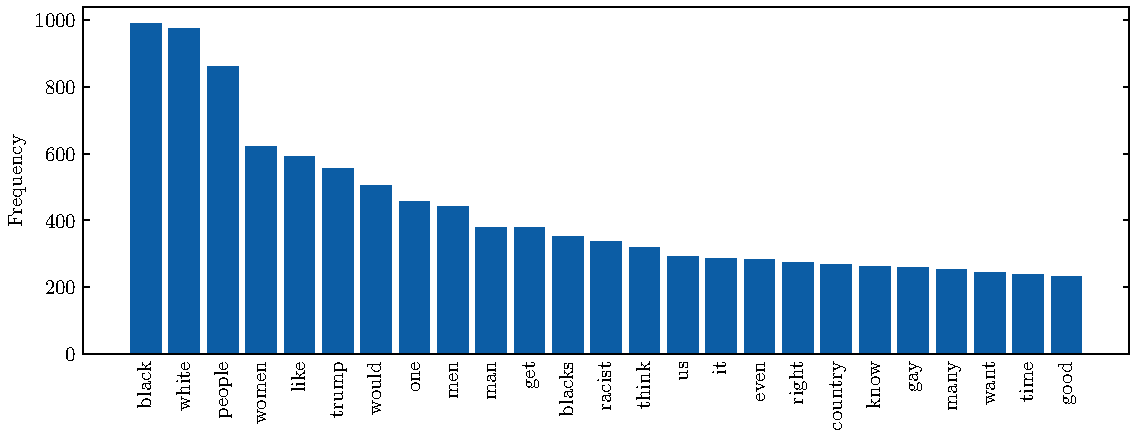
\includegraphics[width=1.0\textwidth]{graphics/toxic_word_freq.pdf}
    \textbf{Notes}: Frequencies represent the number of times an indicated word appears in a comment with a 'toxic' annotation. The top twenty-five most frequent words are labelled.
\end{figure}


\begin{figure}
    \caption{Words appearing most frequently in non-toxic comments}
	\label{fig:non-toxic-word-frequency}
	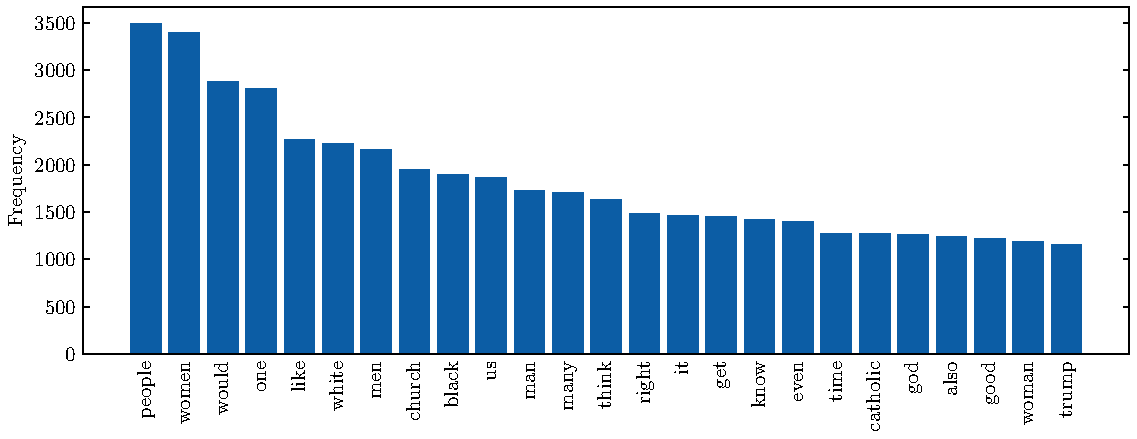
\includegraphics[width=1.0\textwidth]{graphics/nontoxic_word_freq.pdf}
    \textbf{Notes:} Frequencies represent the number of times an indicated word appears in a comment with a 'non-toxic' annotation. The top twenty-five most frequent words are labelled.
\end{figure}